%	INF219
%	Oskar L. F. Lerivåg
%	3D Printer Tizen-wearable application

\documentclass[a4paper, 12pt]{article}

%Bookmarks
\usepackage[colorlinks=true,urlcolor=cyan,linkcolor=black,citecolor=red,bookmarksopen=true]{hyperref}
\usepackage{bookmark}

\usepackage[utf8]{inputenc}
\usepackage{amsmath}
\usepackage{pgf,tikz}
\usepackage{mathrsfs}
\usepackage{listings}
\usetikzlibrary{arrows}
\usepackage{amssymb}
\usepackage{url}

%Images%
\usepackage{graphicx}
\usepackage{float}

%Margins
\usepackage{geometry}
\geometry{a4paper, margin=3cm}

%Citations
\usepackage[round]{natbib}
\bibliographystyle{plainnat}

\newcommand{\mysection}[1]{\section*{#1} \addcontentsline{toc}{section}{#1}}
\newcommand{\mysubsection}[1]{\subsection*{#1} \addcontentsline{toc}{subsection}{#1}}
\newcommand{\mysubsubsection}[1]{\subsubsection*{#1} \addcontentsline{toc}{subsubsection}{#1}}

\newcommand{\mycitation}[1]{[\citet{#1}]}

\begin{document}

    % % % % % % % % % % % % % % % % %
    %
    %	FORDISE!
    %
    %%%%%%%%%%%%%%%%%%%%%%%%%%%%%%%%%%%%%%%%%
% University Assignment Title Page 
% LaTeX Template
% Version 1.0 (27/12/12)
%
% This template has been downloaded from:
% http://www.LaTeXTemplates.com
%
% Original author:
% WikiBooks (http://en.wikibooks.org/wiki/LaTeX/Title_Creation)
%
% License:
% CC BY-NC-SA 3.0 (http://creativecommons.org/licenses/by-nc-sa/3.0/)
% 
% Instructions for using this template:
% This title page is capable of being compiled as is. This is not useful for 
% including it in another document. To do this, you have two options: 
%
% 1) Copy/paste everything between \begin{document} and \end{document} 
% starting at \begin{titlepage} and paste this into another LaTeX file where you 
% want your title page.
% OR
% 2) Remove everything outside the \begin{titlepage} and \end{titlepage} and 
% move this file to the same directory as the LaTeX file you wish to add it to. 
% Then add \input{./title_page_1.tex} to your LaTeX file where you want your
% title page.
%
%%%%%%%%%%%%%%%%%%%%%%%%%%%%%%%%%%%%%%%%%

%----------------------------------------------------------------------------------------
%	PACKAGES AND OTHER DOCUMENT CONFIGURATIONS
%----------------------------------------------------------------------------------------


\begin{titlepage}


    \newcommand{\HRule}{\rule{\linewidth}{0.5mm}} % Defines a new command for the horizontal lines, change thickness here

    \center % Center everything on the page

    %----------------------------------------------------------------------------------------
    %	HEADING SECTIONS
    %----------------------------------------------------------------------------------------

    \textsc{\LARGE Universitetet i Bergen}\\[1.5cm] % Name of your university/college
    \textsc{\Large INF219}\\[0.5cm] % Major heading such as course name
    \textsc{\large Project in informatics I}\\[0.5cm] % Minor heading such as course title

    %----------------------------------------------------------------------------------------
    %	TITLE SECTION
    %----------------------------------------------------------------------------------------

    \HRule \\[0.4cm]
    { \huge \bfseries 3D Printer Tizen-wearable application}\\[0.4cm] % Title of your document
    \HRule \\[1.5cm]

    %----------------------------------------------------------------------------------------
    %----------------------------------------------------------------------------------------
    %	AUTHOR SECTION
    %----------------------------------------------------------------------------------------
    \Large \emph{Authors:}\\
    Oskar Leirvåg (OLE006)
    \\[2cm] % Your name
    %----------------------------------------------------------------------------------------
    \centerline{
\includegraphics[scale=0.15]{figures/canvas}} % Include a department/university logo - this will require the graphicx package
    %----------------------------------------------------------------------------------------
    %	DATE SECTION
    %----------------------------------------------------------------------------------------

    {\large \today}\\[3cm] % Date, change the \today to a set date if you want to be precise

    %----------------------------------------------------------------------------------------
    %	LOGO SECTION
    %----------------------------------------------------------------------------------------

    \vfill
    % Fill the rest of the page with whitespace

\end{titlepage}

    %Table of contents
    \pdfbookmark{\contentsname}{toc}
    \tableofcontents

    %Tving ny side
    \newpage


    % % % % % % % % % % % % % % % % %
    %
    %	Abstract
    %
    \mysection{Abstract}
    {
    This report is meant to summarize everything I have personally learned or experienced during a project in which
    I try to develop an application for the \i{"Samsung Galaxy Watch"} using their proprietary development-studio
    \i{Tizen studio} to allow control of my personal FDM-3D-Printer.
    }
    \newpage

    \mysection{Terminology}
    {
    \mysubsection{Printer parts}
    \begin{itemize}
        \item Extruder: The heated part of the printer which melts the plastic and extrudes it.
        \item Heatbed/printbed: The plate on which a print begins, often heated for better adhesion.
        Also comes in different materials like glass or PEI.
        \item Einsy/motherboard: The main electrical board of the printer which everything is connected to.
        \item Filament: The name of the material used to create models, in a continuous string on a spool.
        Usually made of either plastic or nylon, the most common types are PLA, ABS, PET-G, TPU, and PA-12 which holds
        their unique properties, print-settings, and prices.
    \end{itemize}

    \mysubsection{Technical}
    {
    \begin{itemize}
        \item GCODE: The name of the instructions given to the 3D-Printer and \; is comments.
        These codes refer to single operations eg. \i{M104 S215 \; set extruder temp}.
        GCODE might also refer to GCODE-file. \mycitation{reprap:gcode}
        \item GCODE-file: A file containing up to several hundred-thousand lines of GCODE commands.
        Usually one file per print-job.
        \item Slicer: A program/application which creates a GCODE-file that prints a digital 3d-object.
        Also handles settings like temperature and speeds.
        \item Mesh: A digital file format method for 3d-objects.
        \item STL/OBJ: The some of the most used digital file formats for the mesh method.
    \end{itemize}
    }
    }
    \newpage

    % % % % % % % % % % % % % % % % %
    %
    %	What is this software
    %
    \mysection{What is 3D-Printing}
    {
    \centerline{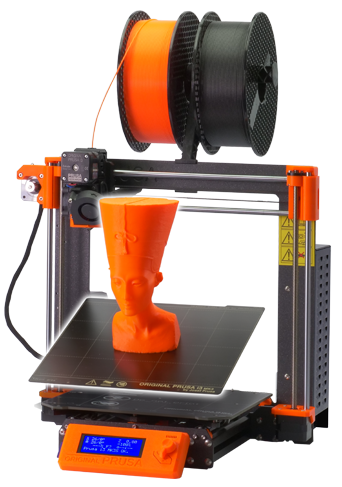
\includegraphics[scale=0.5]{figures/MK3s-home-new}}
    \begin{quote}
        "Any sufficiently advanced technology is indistinguishable from magic." \mycitation{wikiquote:ArthurCClarke}
    \end{quote}

    \mysubsection{The technology}
    {
    3D-Printing is a relative new technology which allows production of computer-designed three-dimensional models
    in certain materials.
    There are many different methods of 3D-Printing like SLS, SLA, DLP and others, but the far most common for home use is FDM,
    which is the type used in this project.
    \\\\
    FDM stands for Filament-deposition-modeling\; a method which extrudes thin strings of plastic in layers as thin as
    0.05mm and up to 1mm, controlled by CNC(computer numeric control).
    This allows the creation of models with great detail and low cost, with the accuracy of stepper-motors.
    It allows to re-use the commands and produce almost exact replicas of the same digital objects with little to no extra
    work.
    \\\\
    Unfortunately this is a tedious process which can take several hours or even days.
    There is little to no control element for the result, while there are countless factors which plays a role for
    the result of a single print.
    Also if an error occurs there is probably no way to recover and you have to start over.
    Luckily the technology is getting better, and more sensors has been added, like filament-runout, and collision detection.
    Alas it is still recommended that you stand by the machine for the entirety of the print, while people still leave their
    homes with the dishwasher running.

    \mysubsubsection{Continuous innovation}
    {
    Computer technology is constantly moving forward, and 3D-Printing is no exception.
    Updates are rolling out continuously for all the different systems, some updates even fix 3.
    party integration problems.
    \\\\
    What really changes 3D-Printer updates is the possibility of sending digital physical upgrades, which you can print
    and change yourself.
    This enables larger beta-testing, cheaper and faster physical upgrading, and shorter production testing before a unit can ship.
    \\\\
    During this project the development-printer has received
    \begin{itemize}
        \item 2 physical updates
        \item 1 physical major version upgrade, requiring some new manufacturer parts
        \item 2 personal modifications for the project
        \item 5 software updates (and 1 personally compiled pre-release to fix project issue) \mycitation{prusa:github:versions}
    \end{itemize}
    }
    }

    \mysubsection{Octoprint}
    {
    As of now, many 3D-Printers are open-source, which allows users to create their own tools and better the control they have.
    One such tool is \i{Octoprint}, which runs on a raspberry-Pi, hosting a web interface for your 3d printer.
    \\\\
    This allows the user to read live sensor data from a web-interface, connect a camera, and even add plugins for more advanced control.
    Allowing such an expansion can ease large manufacturing by eg.
    allowing the removal of a single part that has failed without having to stop the print and loose it entirely.
    \\\\
    Octoprint is tackling many common features requested by 3D-printer companies, and hosting them available under the same
    service.
    This includes web-based automatic slicer, visualization of bed leveling, remote control of axis and temperature, and live camera streaming.
    All this works as both reliability and safety measures for a user, but 3D-Printing is still very complicated and requires
    training and experience for success.
    \\\\
    Octoprint has without a doubt added safety to printing, but is for now only available trough a web-browser,
    with little to no support for smaller screens without plugins.
    Luckily they have a REST-API available, and allows for further development.
    Already there are multiple applications made for the different mobile devices, but less is available for the wearable market.
    }

    \mysubsection{REST-API}
    {
    \mycitation{restfulapi}
    }

    \mysubsection{My Tools}
    {
    During this project several different tools have been used.
    This is the complete list with a short description
    \begin{itemize}
        \item GIT: Version control tool used to track any changes in any documentation or source-code created
        \item Github: Version control provider needed to use GIT, which also holds extra tools for development and issue-tracking.
        As a bonus this is also where both Octoprint and Prusa-Firmware is hosted.
        \item Intellij WebStorm: An IDE for web development, also supports LaTeX with plugins.
        Main development studio due to all the tools it provides.
        \item Tizen IDE: The main development studio has to be used for certificate management, emulator, and device-management.
        \item Google-Chrome: The main browser used for development.
        \item Arduino build tools: Used to compile the firmware for the 3d-printer
        \item Windows 10: Main development OS
        \item Arch-Linux: Secondary linux-distro development, test and deploy OS
        \item Raspbian: Light linux-distro OS needed to host octoprint and control the printer.
        \item Octoprint: A web-service to control open-source 3D-Printers with a web interface.
        Also holds the API and is the tool which will be developed towards.
    \end{itemize}
    }

    \mysubsection{The infrastructure}
    {
    The 3D-Printer only support GCODE commands using mostly the NIST RS274NGC Interpreter \mycitation{reprap:nist}.'
    This requires GCODE to either be supplied trough a SD-card directly in the 3D-Printer or by a physical connection.
    This is where Octoprint is connected.
    Octoprint is running on a RaspberryPi 3B+ using the Raspbian-Lite OS, in a custom built casing on the printer.
    This creates a small computer with a physical connection, and since Octoprint is accessible trough the web-interface
    it acts like a wireless bridge.
    \\\\
    Octoprint is running it's own web-service and allows certain operations even if the printer is turned off.
    It also hosts an Application-protocol-interface which allows other applications to access and use octoprint as a
    service-point connecting to the printer.
    This is how the mobile apps connect, and where the new application will connect.
    }

    }

    %Tving alltid til ny side
    \newpage
    %Laster inn referanser
    \bibliography{citation-db}
    %Legg inn i contents (toc)
    \addcontentsline{toc}{section}{References}

\end{document}